\section{
  Vertical shear instability with dust}\label{results} 

We now present numerical solutions for vertically stratified,
non-self-gravitating disks, assuming perfectly coupled dust. 
We formally take $\tstop=0$ so the equilibrium defined in \S\ref{eqm} 
are exact steady states. In reality,   
%\subsection{Validity}
%{\bf maybe incorporate into intro to this section?}
%We considered $\tstop=0$ in order to perform stability analysis on an
%exact steady state. 
%When $\tstop\neq0$, a stratified dusty 
%disk initialized as in \S\ref{eqm} would evolve 
%as 
dust settles to the midplane on a timescale $t_\mathrm{settle}\sim 
1/\tstop\OmK^2$ \citep{takeuchi02}. However, we expect the 
perfectly-coupled limit to be valid  
provided timescales of interest $t_\mathrm{grow}\ll
t_\mathrm{settle}$. For the VSI this translates to 
%Since VSI growth rates are $O(h_\mathrm{g}\OmK)$, 
%we require  
%\begin{align}
 $ \tstop\OmK \ll h_\mathrm{g}. $
%\end{align} 
For thin PPDs, this is satisfied for $\tstop\OmK \ll O(10^{-2})$.   


We first consider constant
midplane dust-to-gas ratios $\epsilon_0$ and characteristic thickness
$H_\epsilon$. Then the dust-to-gas ratio $\epsilon=\epsilon(z)$. In 
this limit any growing modes must be associated with the imposed
temperature gradient (see \S\ref{limits}). We are then studying the
effect of dust-loading on the VSI previously studied in pure gas
disks \citep[][\citetalias{lin15} in this section]{lin15}. In 
\S\ref{varHd} we allow $\p_r\epsilon\neq 0$, and in 
\S\ref{vert_mixed} we consider VSI driven entirely by radial
gradients in the dust-to-gas ratio (as discussed in
\S\ref{iso_perfect}).  

The parameters for the linear problem includes $\epsilon_0$, the dust
layer thickness $\Hd$, and the perturbation radial wavenumber
$k_x$. We choose a midplane gas density profile 
$\rho_\mathrm{g0}\propto r^{-3/2}$. The fiducial power-law 
index for the temperature profile is $q=-1$; and we set the gas disk
aspect-ratio $h_\mathrm{g}=0.05$. These values were also used by  
\citetalias{lin15}. 

%Two boundary conditions are needed for the $\tstop=0$
%problem \citep[e.g.][]{lubow93}. 
We impose solid vertical boundaries so that $\delta
v_z(\pm\zmax)=0$. We solve the linearized equations as a generalized
eigenvalue problem using a pseudo-spectral code adapted  
from \citetalias{lin15}. Amplitudes are expanded in Chebyshev
polynomials up to order $512$. %We check results using
%Eq. \ref{vsi_check}.      

\subsection{Qualitative expectations}\label{vsi_est}
\citetalias{lin15} found the appropriate way to compare 
vertical shear (destabilizing) and  vertical buoyancy (stabilizing)
is $r\p_z\Omega/\OmK$  against $N_z^2/\OmK^2$. From 
\S\ref{vertshear} and \S\ref{vbuoyancy} we find $|r\p_z\Omega|\sim q
h_\mathrm{g}\OmK$ for a 
thin, gas dominated disk; while $N_z^2\sim \epsilon\OmK^2$. Thus we
expect dust-induced buoyancy forces to stabilize the disk against the
VSI where $\epsilon \gtrsim h_\mathrm{g}$. 

%\begin{align}

\subsection{Effect of dust-loading}
We first vary the midplane dust-to-gas ratio 
$\epsilon_0\in[10^{-3},1]$, fixing the dust thickness to  
$\Hd=0.99\Hg$. Then  $\epsilon$ is roughly constant with height. We
set the vertical domain to $\zmax=5\Hg$.  

Fig. \ref{compare_vshear_fixHd} compares the basic state
vertical shear rate, which is destabilizing, and the vertical buoyancy
frequency, which is stabilizing. For the nearly dust-free disk
$\epsilon_0=10^{-3}$ the vertical shear dominates buoyancy for all
$|z|>0$. However, a heavy dust-load with $\epsilon_0=1$ renders the 
buoyancy to dominate over vertical shear in the disk atmosphere 
$|z|\gtrsim 2.5\Hg$. We thus expect instability all heights for 
$\epsilon_0=10^{-3}$, but to be restricted to the midplane for
$\epsilon_0=1$. 

\begin{figure}
  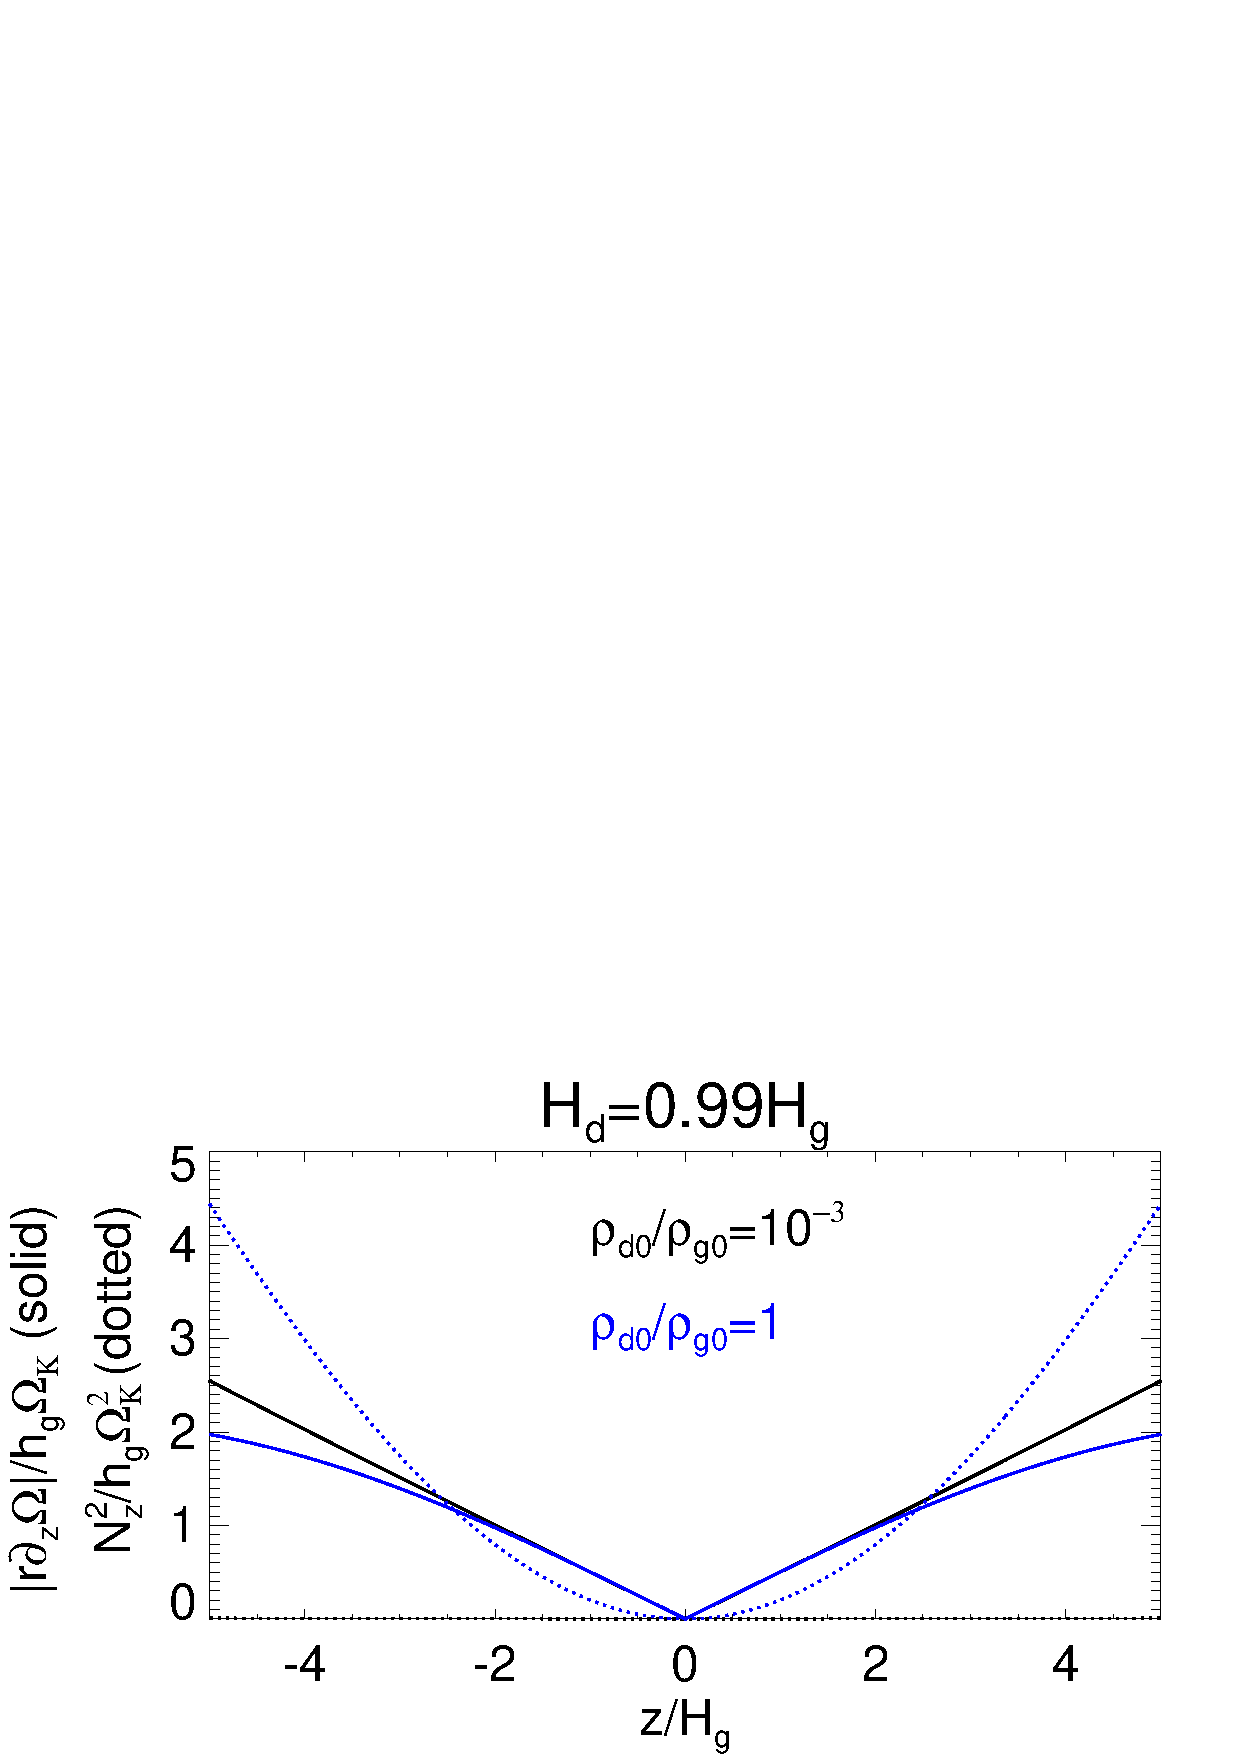
\includegraphics[width=\linewidth]{figures/compare_vshear_Nz2_fixHd} 
  \caption{Vertical shear rate (solid) compared to vertical buoyancy
    (dotted) in a locally isothermal, dusty disk with midplane dust-to-gas ratio
    of $\epsilon_0=10^{-3}$ (black) and $\epsilon_0=1$ (blue). 
    The dust layer thickness is fixed to $\Hd=0.99\Hg$ so the 
    dust-to-gas ratio $\epsilon$ is approximately constant with
    height. Vertical buoyancy here is due to dust-loading. 
    \label{compare_vshear_fixHd}
    }
\end{figure}

Fig. \ref{vsi_dust_loading} show unstable modes for different values
of $\epsilon_0$ with fixed perturbation wavenumber  $k_x\Hg = 30$. The
eigenvalue distributions for $\epsilon_0 \leq 10^{-2}$ are similar to the
dust-free fiducial case considered by \citetalias{lin15}. This is
expected since $\epsilon_0 < \hgas$ (\S\ref{vsi_est}). Eigenvalues 
consists 
of the roughly horizontal `body modes', and the nearly-vertical
`surface modes' \citep[which are associated with the imposed vertical
boundaries, ][]{barker15}.   

We find that increasing the dust-to-gas ratio reduce VSI growth
rates. Notably, surface modes, which are typically fastest growing in
the dust-free case, are suppressed in dusty disks for $\epsilon_0\geq
0.1$ (i.e. $\epsilon_0> \hgas$).   
The body modes' growth rates remain $ O(h_\mathrm{g}\OmK)$ 
but their oscillation frequency increases with
dust-loading, i.e. it increases with the vertical buoyancy. 
The total number of modes do not change 
significantly. This is in contrast with the effect of increasing
cooling times in an adiabatic gas disk, for which \citetalias{lin15}
find fewer unstable modes. 
%until the system is eventually completely stable. 

\begin{figure}
  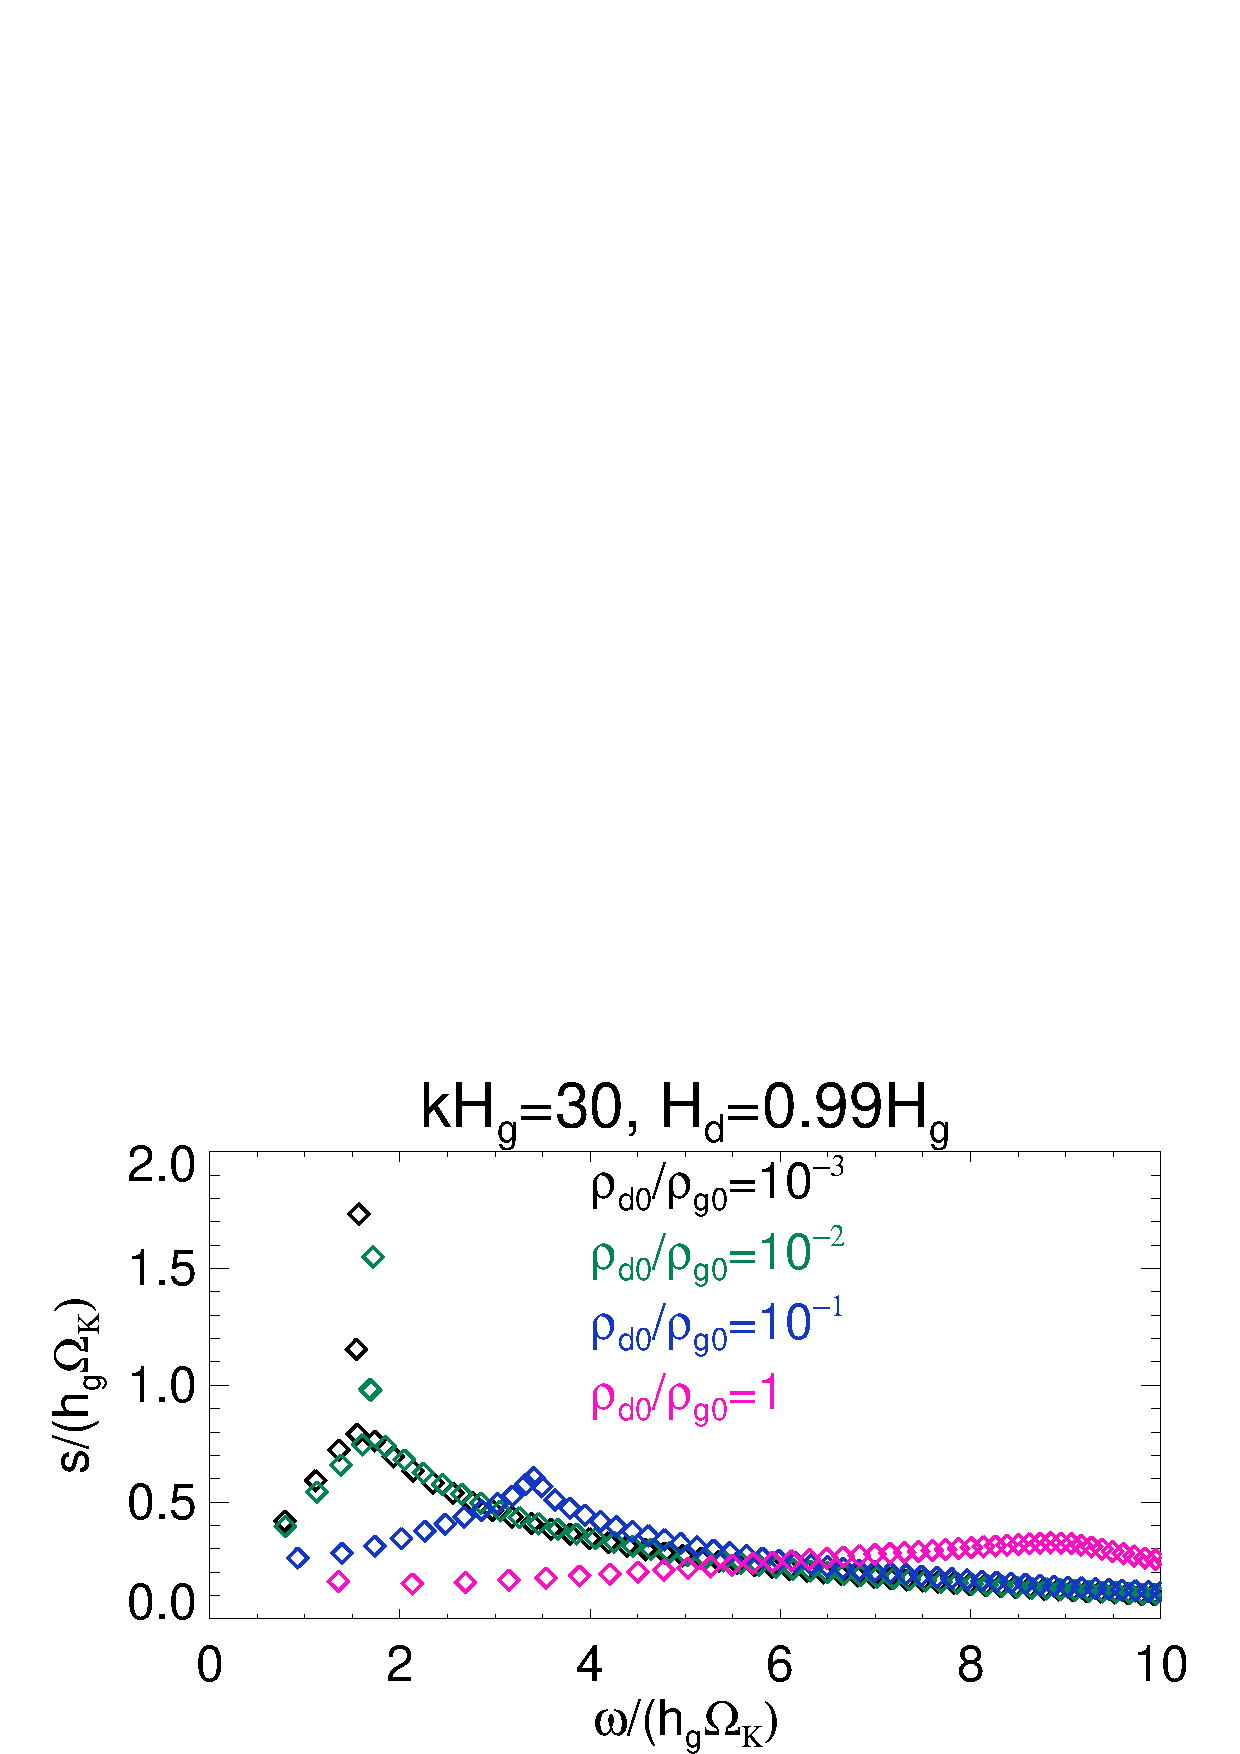
\includegraphics[width=\linewidth]{figures/compare_eigenvals_kx30Hd1} 
  \caption{Unstable modes in a locally isothermal, perfectly coupled
    dusty disk with fiducial parameters
    $(p,q,h_\mathrm{g}, \Hd/\Hg )=(-1.5,-1,0.05, 0.99)$. The real
    frequency $\omega$ and growth rates $s$ are shown for a range of
    midplane dust-to-gas ratios $\epsilon_0=\rho_\mathrm{g0}/\rho_\mathrm{d0}$. 
    \label{vsi_dust_loading}
    }
\end{figure}

The lowest frequency `fundamental' body mode is energetically dominant
because the entire disk column is perturbed \citep[cf. surface modes
  which only disturb the disk boundaries,][]{umurhan16c}. In Fig. \ref{vsi_dust_loading2d}
we compare the fundamental mode between the nearly 
dust-free case $\epsilon_0=10^{-3}$ an a dusty disk with
$\epsilon_0=1$. Dust-loading preferentially
stabilizes the disk atmosphere against the VSI, restricting
meridional motions to $|z|\lesssim 2\Hg$. 
This is consistent with Fig. \ref{compare_vshear_fixHd} comparing the basic state vertical
shear and buoyancy. % Notice also maxium perturbtions to the dust-to-gas ratio,
% $\delta\epsilon$, shifts from disk boundaries 
% to the midplane.  

\begin{figure}
%  \includegraphics[scale=0.54, clip=true, trim=0cm 2.5cm 0cm 0cm]{figures/result2d_dg1d-3.ps}\\
%  \includegraphics[scale=0.54]{figures/result2d_dg1.ps} 
\includegraphics[scale=0.32, clip=true, trim=0.5cm 0cm 3cm 0cm]{figures/result2d_dg1d-3.ps}\includegraphics[scale=0.32, clip=true, trim=1.8cm 0cm 0cm 0cm]{figures/result2d_dg1.ps}
  \caption{Fundamental dusty VSI mode in real space for midplane dust-to-gas
    ratio $\epsilon_0=10^{-3}$ (left) and $\epsilon_0=1$
    (right). The color scale shows the perturbation to the
    dust-to-gas ratio, $\delta\epsilon$; and the arrows show
    $\sqrt{\rho}\left(\dd v_x, \dd v_z\right)$. 
    \label{vsi_dust_loading2d}
    }
\end{figure}

In Fig. \ref{vsi_dust_loading_vareps} we plot the growth rates as a
function of $\epsilon_0$ for different perturbation wavenumbers
$k_x$. Dust-loading stabilizes the VSI more effectively for shorter
wavelength perturbations. This is because for high wavenumbers the
dominant modes are surface modes, which are effectively stabilized by
dust-loading as buoyancy forces are largest near the vertical 
boundaries. The figure suggest that VSI becomes much less efficient
for $\epsilon_0\gtrsim 0.1$ and $k_x\Hg\gtrsim 50$. 

\begin{figure}
  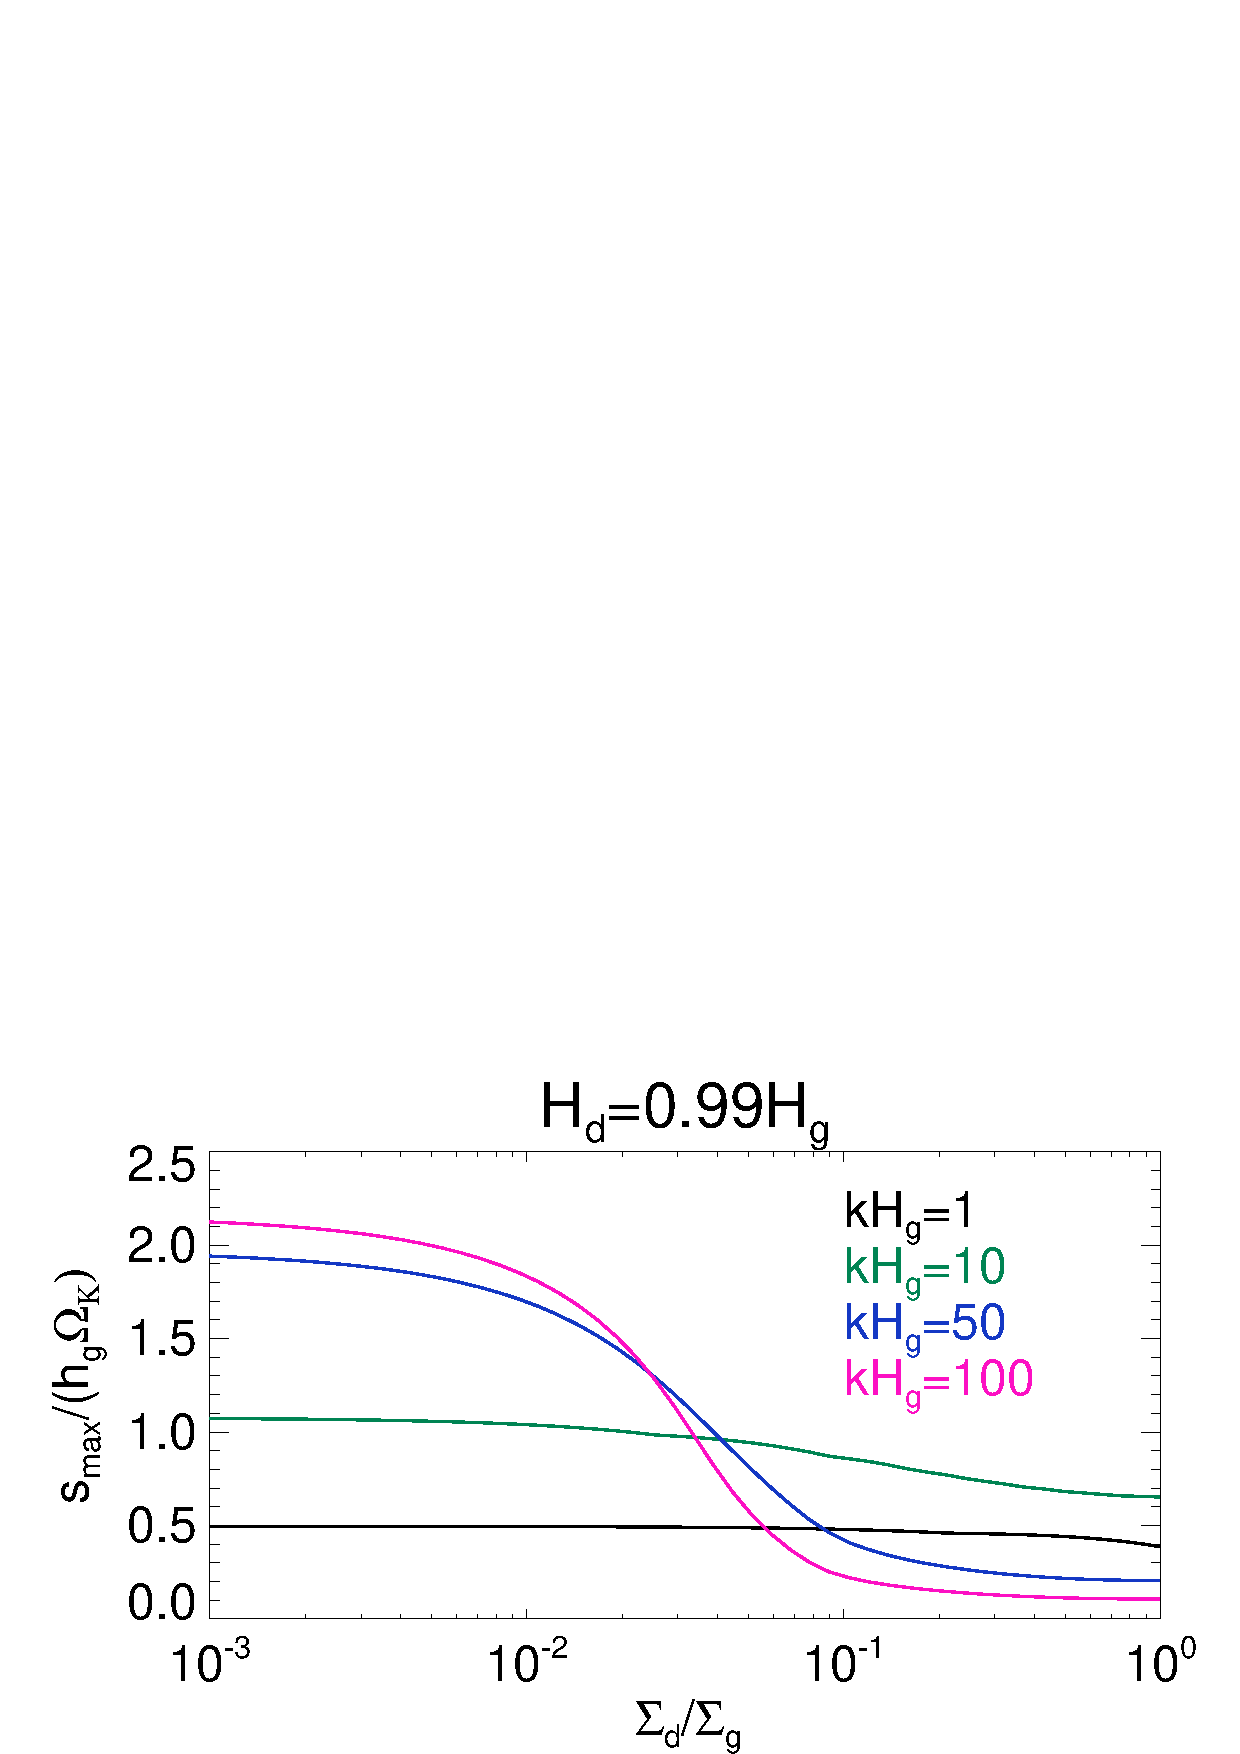
\includegraphics[width=\linewidth]{figures/compare_eigenvals_vareps2} 
  \caption{Maximum growth rate of the dusty VSI as a function of the
    midplane dust-to-gas ratio $\epsilon_0$ for perturbations with
    different radial wavenumbers $k$. The dust layer thickness is
    fixed to $\Hd\simeq \Hg$. 
    \label{vsi_dust_loading_vareps}
    }
\end{figure}




\subsection{Effect of dust layer thickness} 
We now vary $\Hd$ but fix the metalicity 
$Z \equiv \epsilon_0 \Hd/\Hg = 0.03$ to obtain $\epsilon_0$. Since we
will consider thin dust layers, here we use a smaller   
domain with $\zmax=2\Hg$ so that $\epsilon$ does not become
too small. 

We analyze two disks with $\Hd=0.1\Hg$ and 
$\Hd=0.99\Hg$. Fig. \ref{compare_vshear_fixZ} compares the vertical
shear  rate and buoyancy frequency. For $|z|\gtrsim 0.4\Hg$ the two
disks have the same profile with vertical shear dominating over
buoyancy. We thus expect perturbations away from the disk midplane in 
both cases. For $|z|\lesssim 0.4\Hg$, a thin dust 
layer with $\Hd=0.1\Hg$ boosts the vertical shear rate, but the
associated buoyancy is larger still, implying the mid-plane should be
stable. 
%Thus we expect the mid-plane of 
%the disk with $\Hd=0.1\Hg$ to have limited vertical motions.  

\begin{figure}
  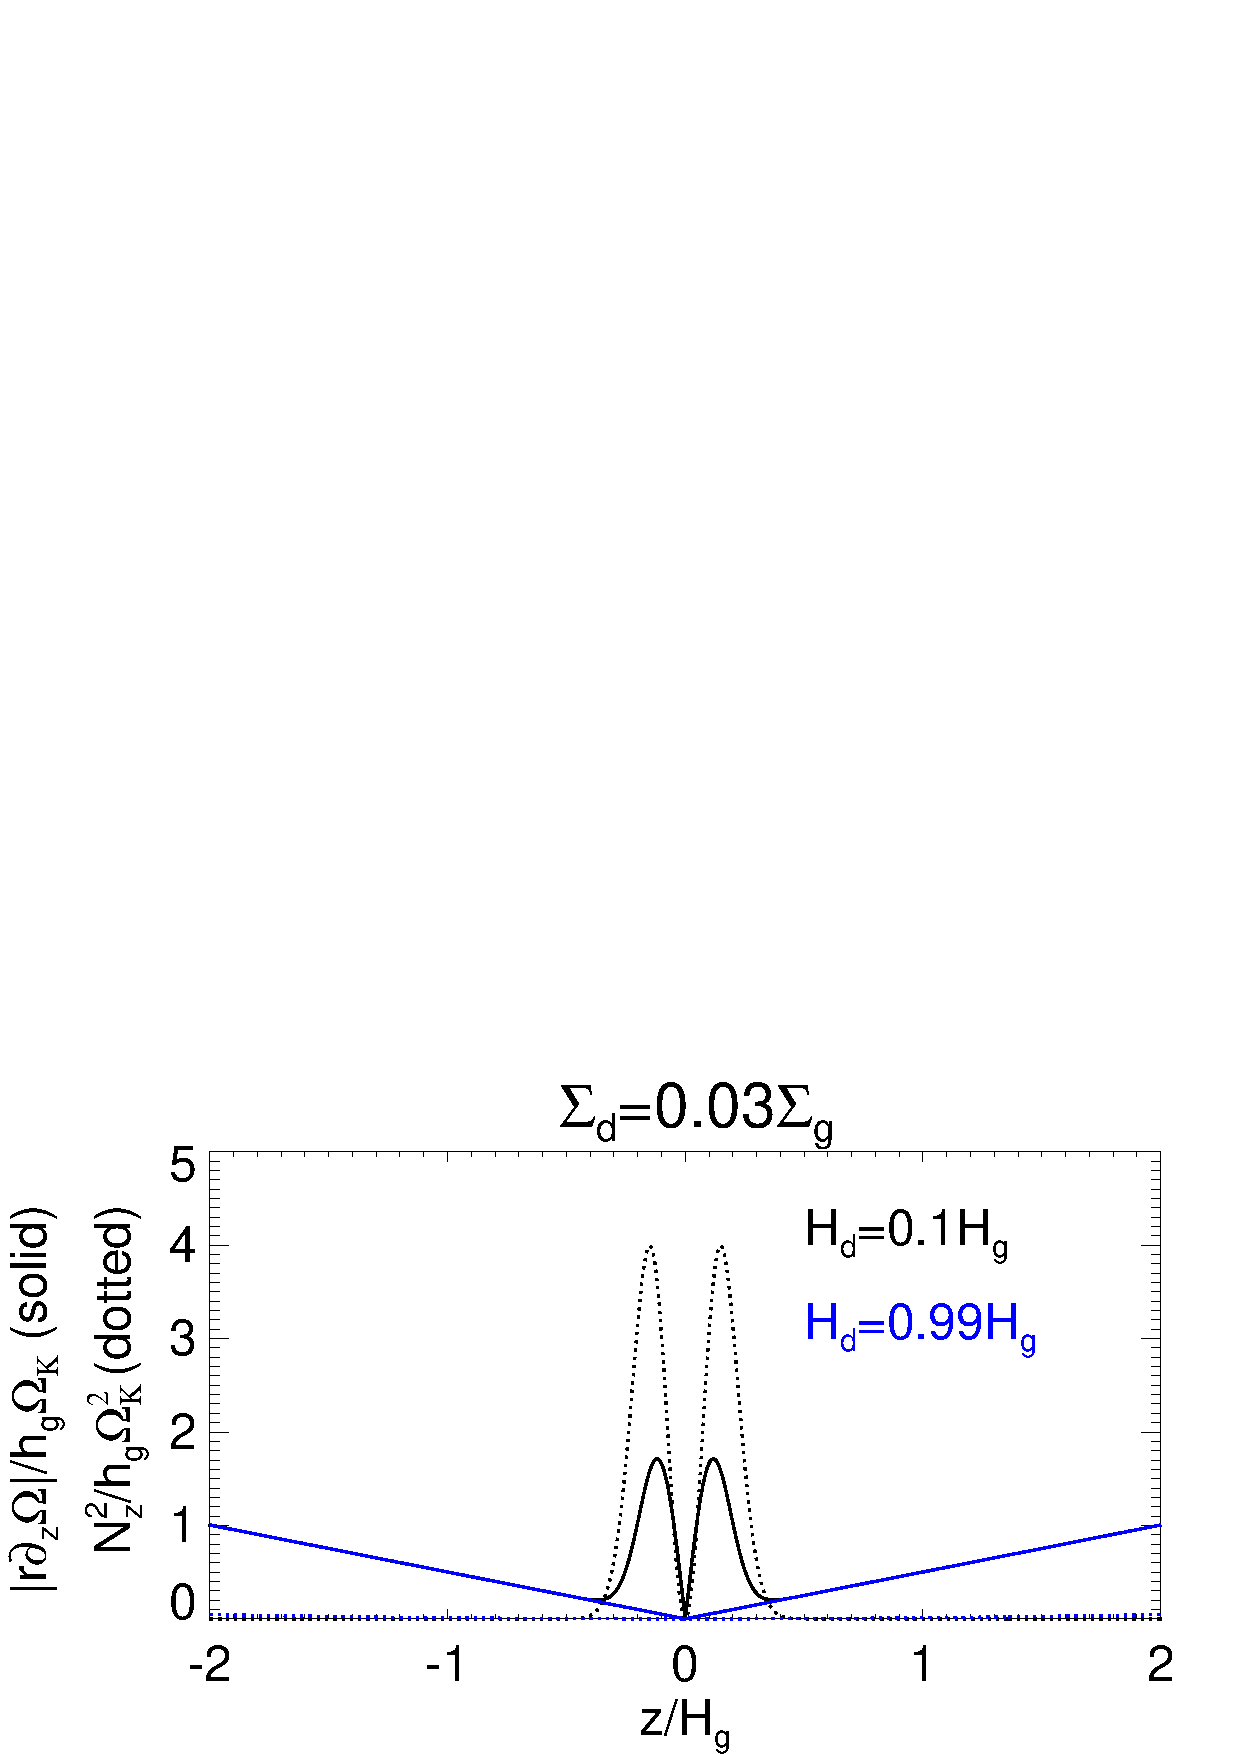
\includegraphics[width=\linewidth]{figures/compare_vshear_Nz2_fixZ} 
  \caption{Vertical shear rate (solid) compared to vertical buoyancy
    (dotted) in a locally isothermal, dusty disk 
    with metalicity $Z=0.03$ and dust thickness $\Hd=0.1\Hg$
    (black) and $\Hd=0.99\Hg$ (blue). 
    \label{compare_vshear_fixZ}
    }
\end{figure}

Fig. \ref{result2d_fixZ} compares the fastest growing VSI body modes  
with $k_x\Hg=30$ for the two cases above.\citepalias[The thinner domain
  adopted here eliminates surface modes, ][]{lin15}.   
We find very similar mode 
frequencies 
\begin{align*}
  \sigma = \begin{cases}
    \left(0.3053\ii - 0.8142\right)h_\mathrm{g}\OmK & \Hd=0.99\Hg, \\
    \left(0.3178\ii - 1.2237\right)h_\mathrm{g}\OmK & \Hd=0.1\Hg,
  \end{cases}
\end{align*}
since the vertical shear profile is similar throughout most of the
disk. However, meridional motions are suppressed near the midplane of
the $\Hd=0.1\Hg$ disk, as expected from the larger buoyancy frequency
relative to vertical shear there. This leads to a structure
analogous to PPD dead zones: a quiescent midplane between active
surface layers \citep{gammie96}.  


\begin{figure}
  \includegraphics[scale=0.32, clip=true, trim=0.5cm 0cm 3cm 0cm]{figures/result2d_Hd1.ps}\includegraphics[scale=0.32, clip=true, trim=1.8cm 0cm 0cm 0cm]{figures/result2d_Hd0d1.ps} 
  \caption{Fastest-growing dusty VSI mode in real space for midplane
    dust layer thickness $\Hd=0.99\Hg$ (left) and $\Hd=0.1\Hg$
    (right). The dust content is fixed to
    $\Sigma_\mathrm{d}=0.03\Sigma_\mathrm{g}$. 
    The color scale shows the perturbation to the
    dust-to-gas ratio, $\delta\epsilon$; and the arrows show
    $\sqrt{\rho}\left(\dd v_x, \dd v_z\right)$.
    \label{result2d_fixZ}
    }
\end{figure}

Fig. \ref{compare_eigenvals_fixZ} shows the maximum VSI growth rates
as a function of $\Hd$. As before, we find growth
rates are most affected by the vertical structure of the dust layer
when the perturbation wavenumer is large. Notice VSI growth rates converge as
$\Hd\to 0$. %to dust free values?    
Thus a thin dust layer, however large its associated vertical shear,
does not affect VSI growth rates. The non-monotonic behavior for $\Hd\gtrsim
0.5\Hg$ arises because the vertical buoyancy frequency 
\begin{align*}
N_z^2(H_d;z,Z) \simeq &Z\Hg z^2
\exp{\left(-\frac{z^2}{2\Hg^2}\right)}\OmK^2\notag\\
&\times 
\frac{1}{\Hd}\left(\frac{1}{\Hd^2} -
\frac{1}{\Hg^2}\right)\exp{\left(-\frac{z^2}{2\Hd^2}\right)}  
\end{align*}
is a non-monotonic function of $\Hd$ at fixed $z$. At $z=\Hg$ and $z=2\Hg$
the buoyancy frequency is maximized for $\Hd\simeq0.5\Hg$ and
$\Hd\simeq 0.8\Hg$, respectively. This is consistent with the abscissa
of minima in growth rates in Fig. \ref{compare_eigenvals_fixZ}. 

\begin{figure}
  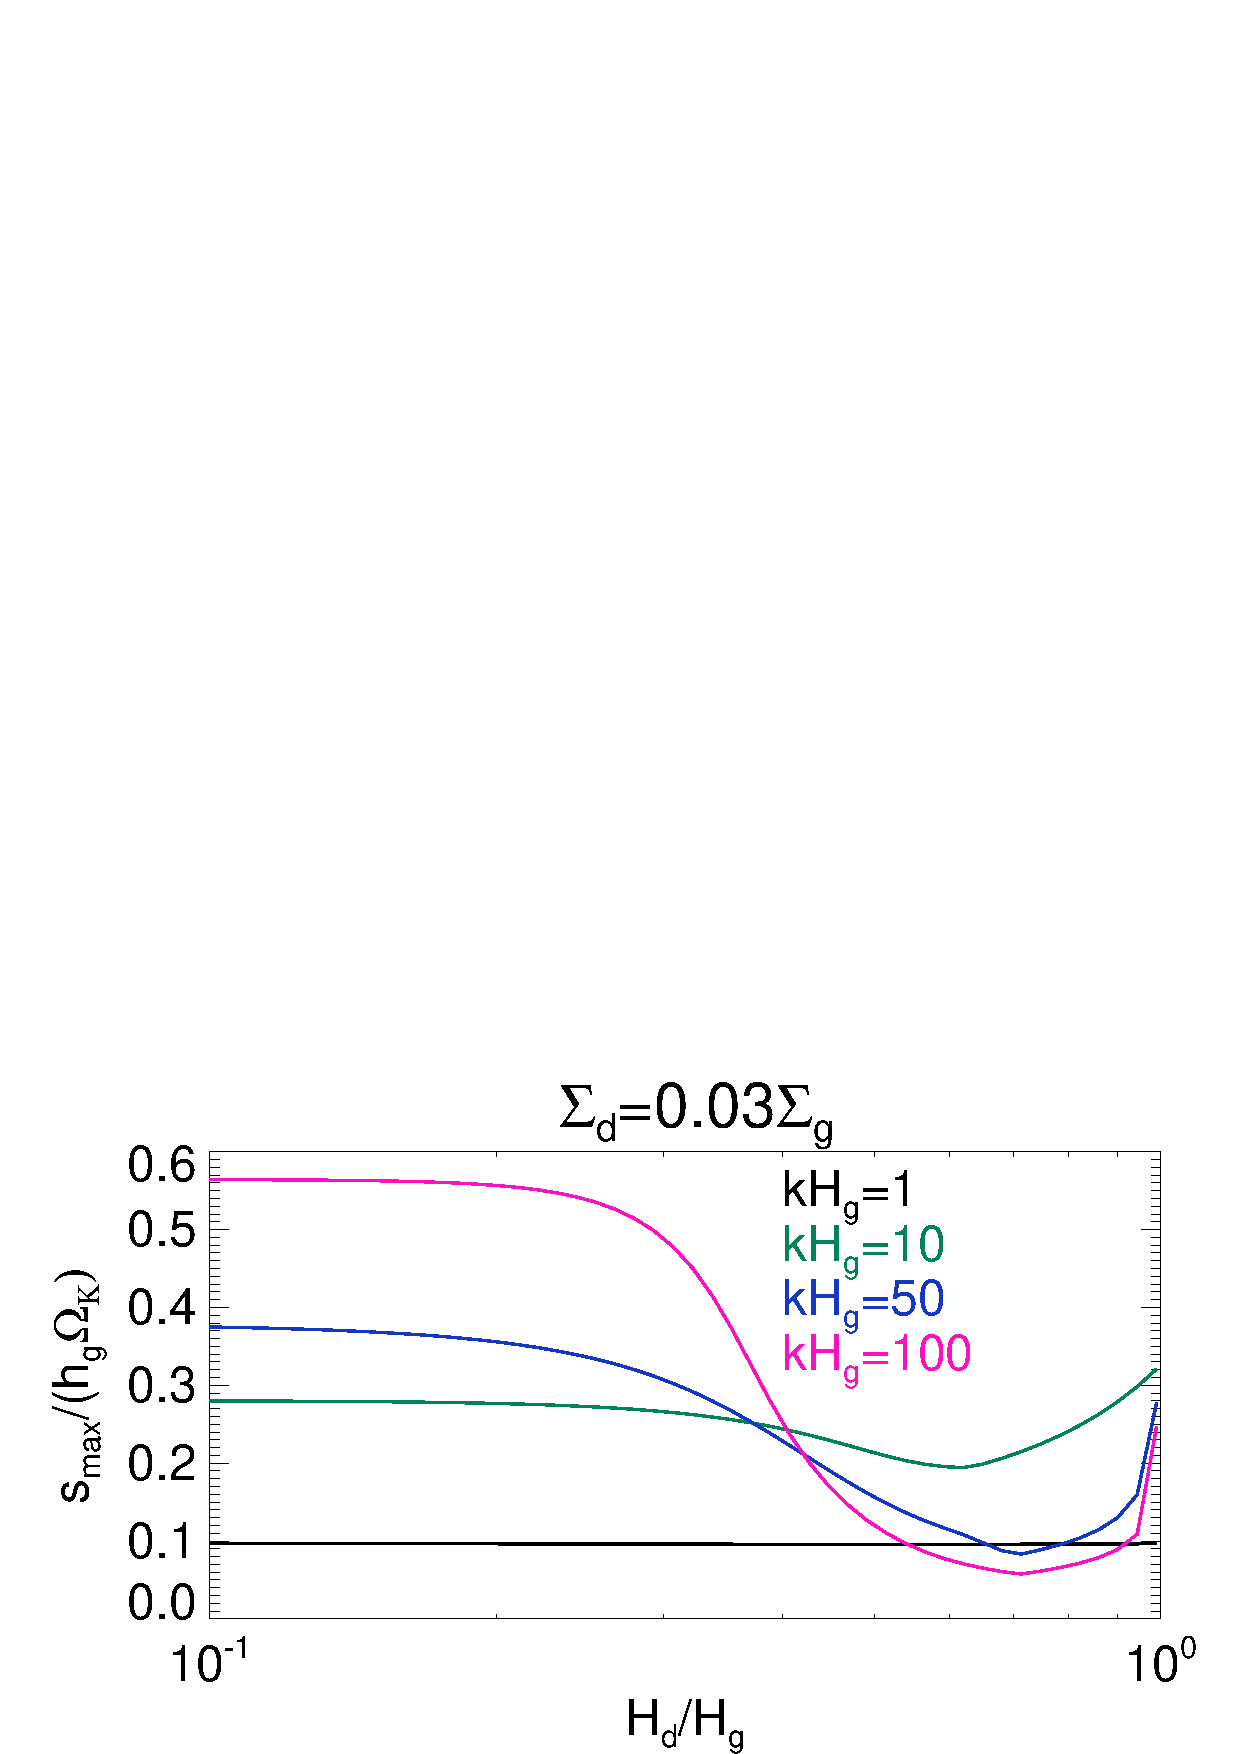
\includegraphics[width=\linewidth]{figures/compare_eigenvals_fixZ} 
  \caption{Maximum VSI growth rate for different perturbation
    wavenumbers $k$ as a function of the dust layer
    thickness $\Hd$ at fixed metalicity $Z=0.03$. 
    \label{compare_eigenvals_fixZ}
    }
\end{figure}

\subsection{Axisymmetric stability of ultra-thin dust layers}
The discussion in \S\ref{iso_perfect} imply strictly  
isothermal disks with a radially uniform dust-to-gas ratio are
stable against axisymmetric perturbations, no matter how thin the dust
layer is. We now demonstrate this numerically. 

To connect with similar studies, here  we also use 
the Richardson number $\rich \equiv N_z^2/\left(r\p_z\Omega\right)^2$
to label calculations \citep{youdin02}.   
Numerical simulations show    
non-axisymmetric instabilities develops when $\rich\lesssim0.1$, brought about
by very thin dust layers \citep{chiang08, lee10}. We show that \emph{axisymmetric}
instabilities never develop in radially uniform disks, however small $\rich$. 

We shall consider ultra thin dust layers with $\Hd\leq 0.01\Hg$ and thus
restrict the vertical domain to $\zmax = 0.02\Hg$. We fix the 
metalicity $Z=0.01$ so the midpane dust-to-gas ratio $\epsilon_0$ is 
$O(1)$.  We consider radial wavenumbers with $k_x\Hd=1$. 

Fig. \ref{ultra_thin} shows the maximum growth rate  as a function of
the radial temperature gradient, $q$. For all cases the vertical
shear is dominated by that due to the dust layer (see
\S\ref{vertshear}). However, we see that $s\propto
|q|$, i.e growth rates vanish in the strictly isothermal limit.  
In particular, this holds for $\rich < 0.1$, the critical value 
for non-axisymmetric instabilities. 

Axisymmetric instability here is associated with the thermal
contribution to vertical shear: as $q\to0$,  $\p_z\Omega$ becomes
entirely due to $\p_z\epsilon$ and there is no instability ($s\to
0$). This result is independent of $\rich$, so the Richardson number
is does not characterize the axisymmetric stability of dust
layers. 

\begin{figure}
  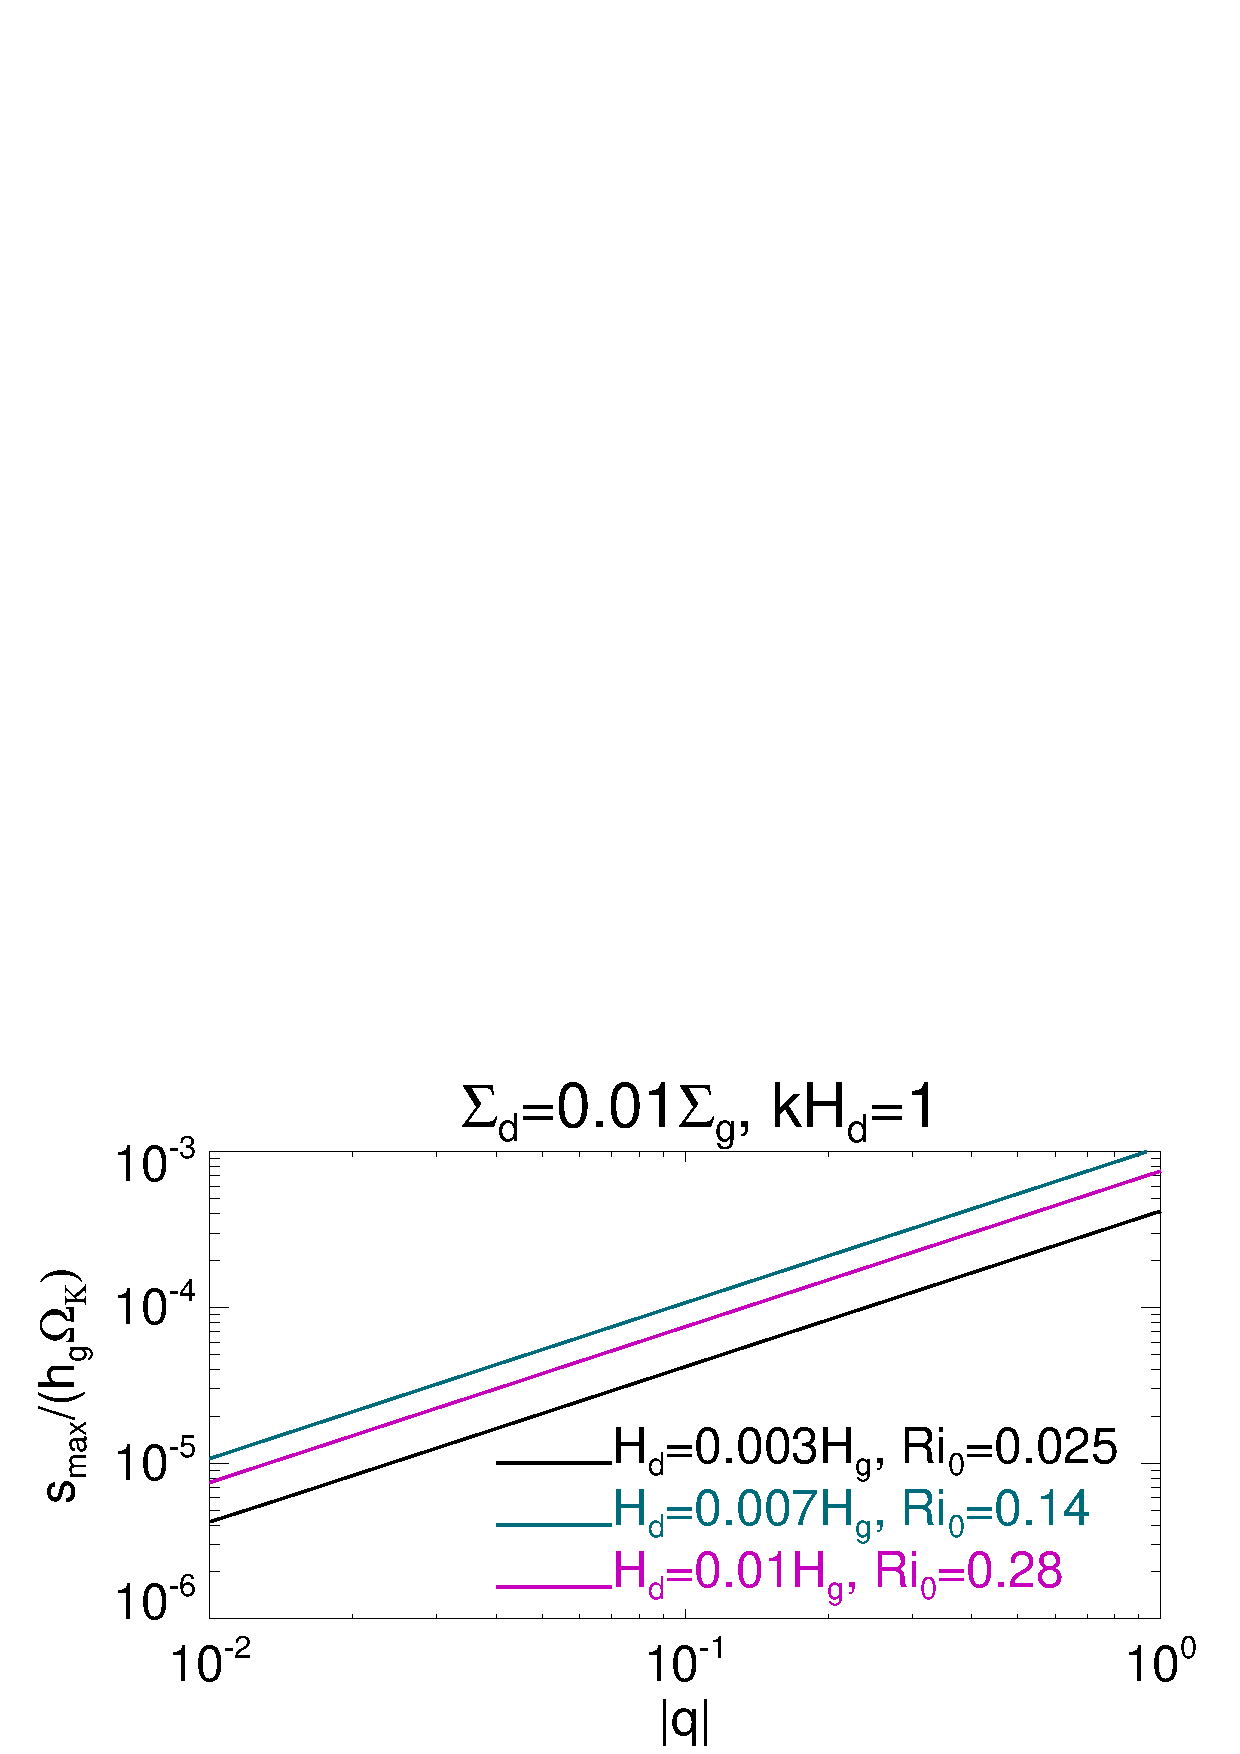
\includegraphics[width=\linewidth]{figures/compare_eigenvals_thindust} 
  \caption{Maximum VSI growth rate for ultra-thin dust layers $\Hd 
    \leq 0.01\Hg$ (with radially uniform dust-to-gas  ratio). Vertical shear is dominated by that due to 
    vertical dust stratification, but axisymmetric instability is still 
    associated with the radial temperature gradient $q$. 
 Here, $\rich_0$ is the minimum 
    Richardson number in the domain in the limit $q\to0$. The disk is stable to axisymmetric perturbations 
    in the strictly isothermal limit, regardless of the dust layer thickness. 
    \label{ultra_thin}
    }
\end{figure}




\subsection{Effect of a radially-varying dust-to-gas ratio}\label{varHd}
%{\bf bonus stuff, maybe delete in final version}

We now consider a radially-varying dust-to-gas ratio. Specifically we
let $\epsilon_0\propto r^{-1}$ and $H_\epsilon \propto \Hg$
(cf. constant values in the previous calculations). Then
\begin{align*} 
  \frac{\p\epsilon}{\p r} =
  \left(\frac{z^2}{H_\epsilon^2}\frac{d\ln{\Hg}}{dr} -
    \frac{1}{r}\right)\epsilon.   
\end{align*}
Here we fix $Z=0.01$, $\Hd=0.8\Hg$.       

Fig. \ref{compare_vshear_varHd} shows that a radially-varying
dust-to-gas ratio increases the magnitude of the vertical shear rate
away from the midplane (see also Eq. \ref{vshear2}). Thus we {
  typically} find higher VSI growth rates, as shown in
Fig. \ref{vsi_dust_varHd}. 
Surfaces modes, { appearing at high $k_x$}, are more effectively
enhanced by the additional vertical shear induced by
$\p_r\epsilon$. { Low frequency body modes with small
  $k_x$ are more affected by radial variations in the 
  dust-to-gas ratio than high-$k_x$, high-frequency body modes. }    

However, all growth rates remain
$O(\hgas\OmK)$. Importantly, the increase in the growth rate of the
fundamental mode is small. We do not expect the radial
dependence in $\epsilon$ to significantly affect the VSI in a dusty
disk. 

\begin{figure}
  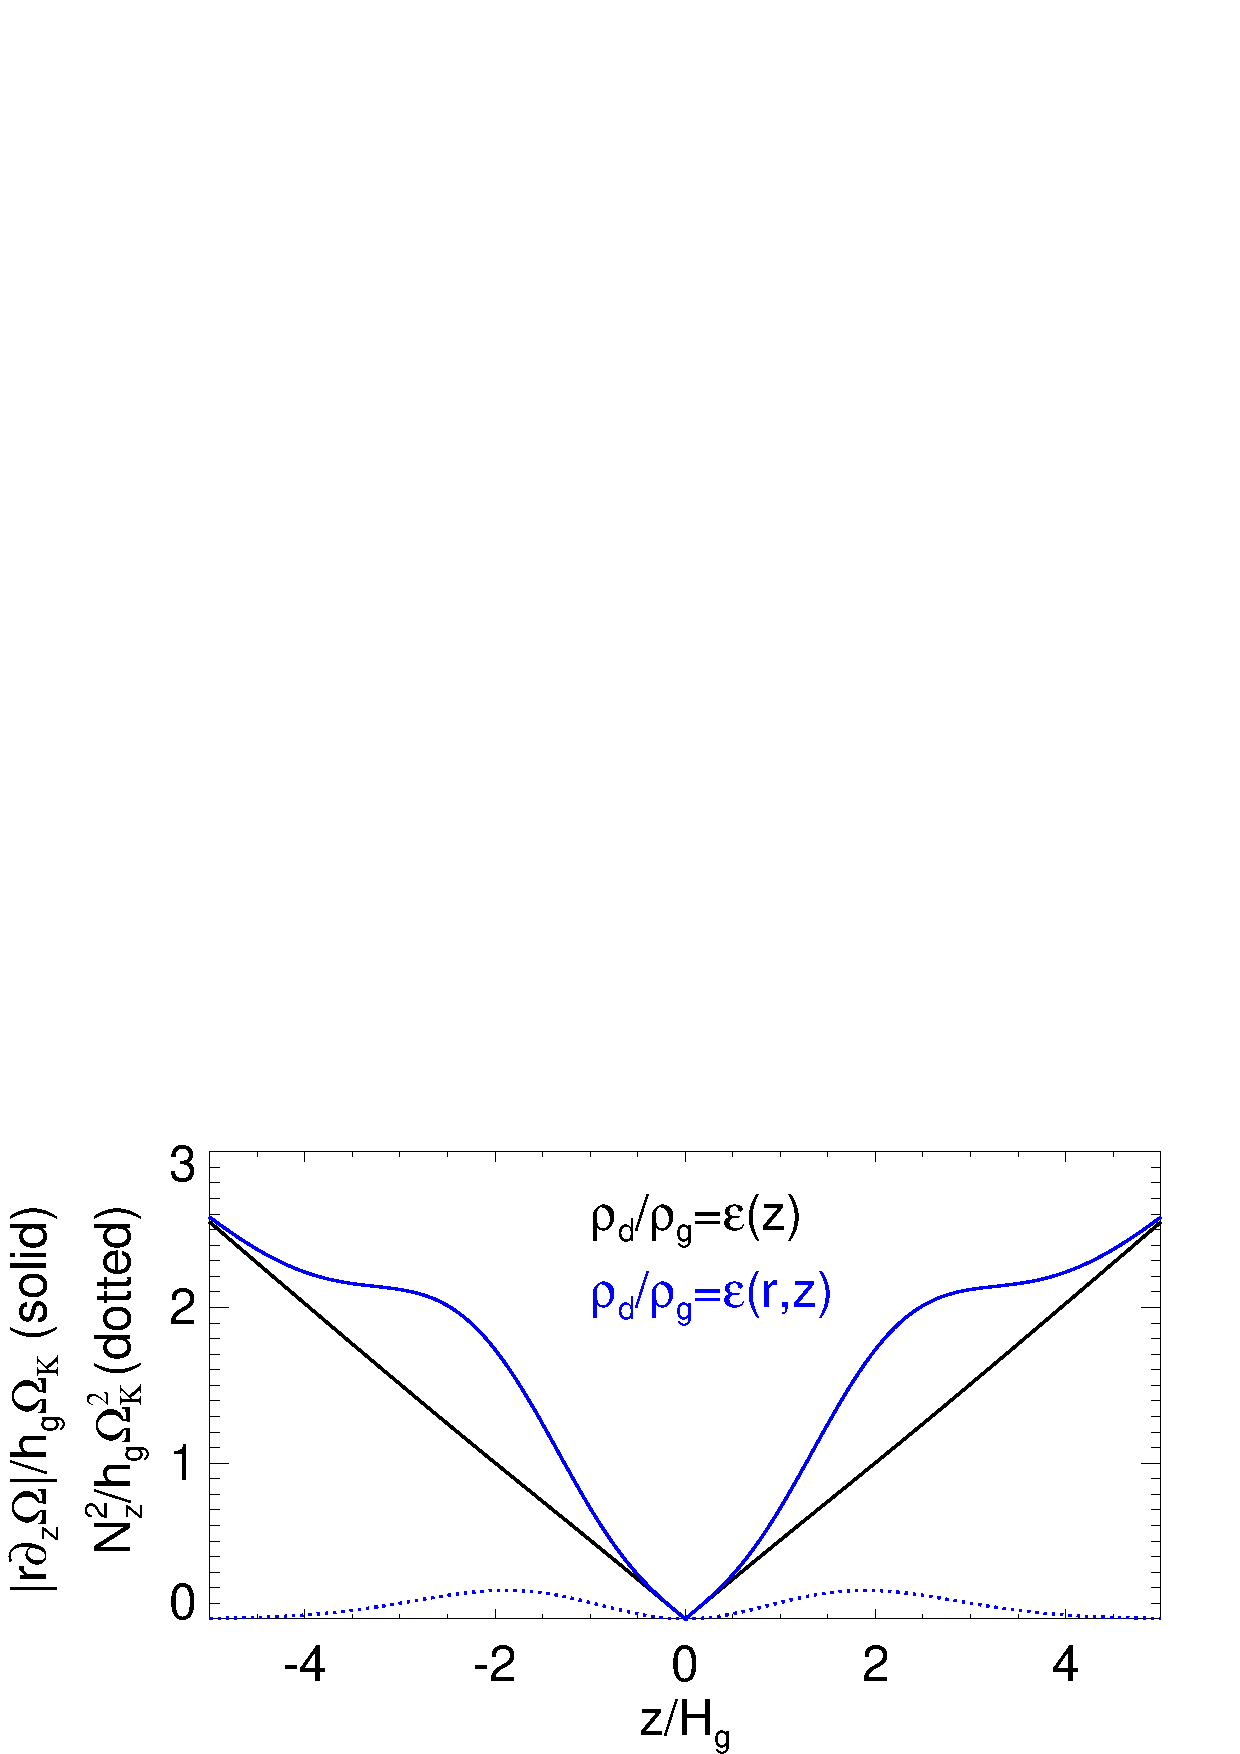
\includegraphics[width=\linewidth]{figures/compare_vshear_Nz2_varHd} 
  \caption{Vertical shear rate (solid) compared to vertical buoyancy
    (dotted) in a locally isothermal, dusty disk 
    with metalicity $Z=0.01$ and dust thickness $\Hd=0.8\Hg$.
    Black curves assume a dust-to-gas ratio that only depends on
    height; whereas the blue curve also allows a radial dependence in
    $\epsilon$. See text for details.  
    \label{compare_vshear_varHd}
    }
\end{figure}



\begin{figure}
  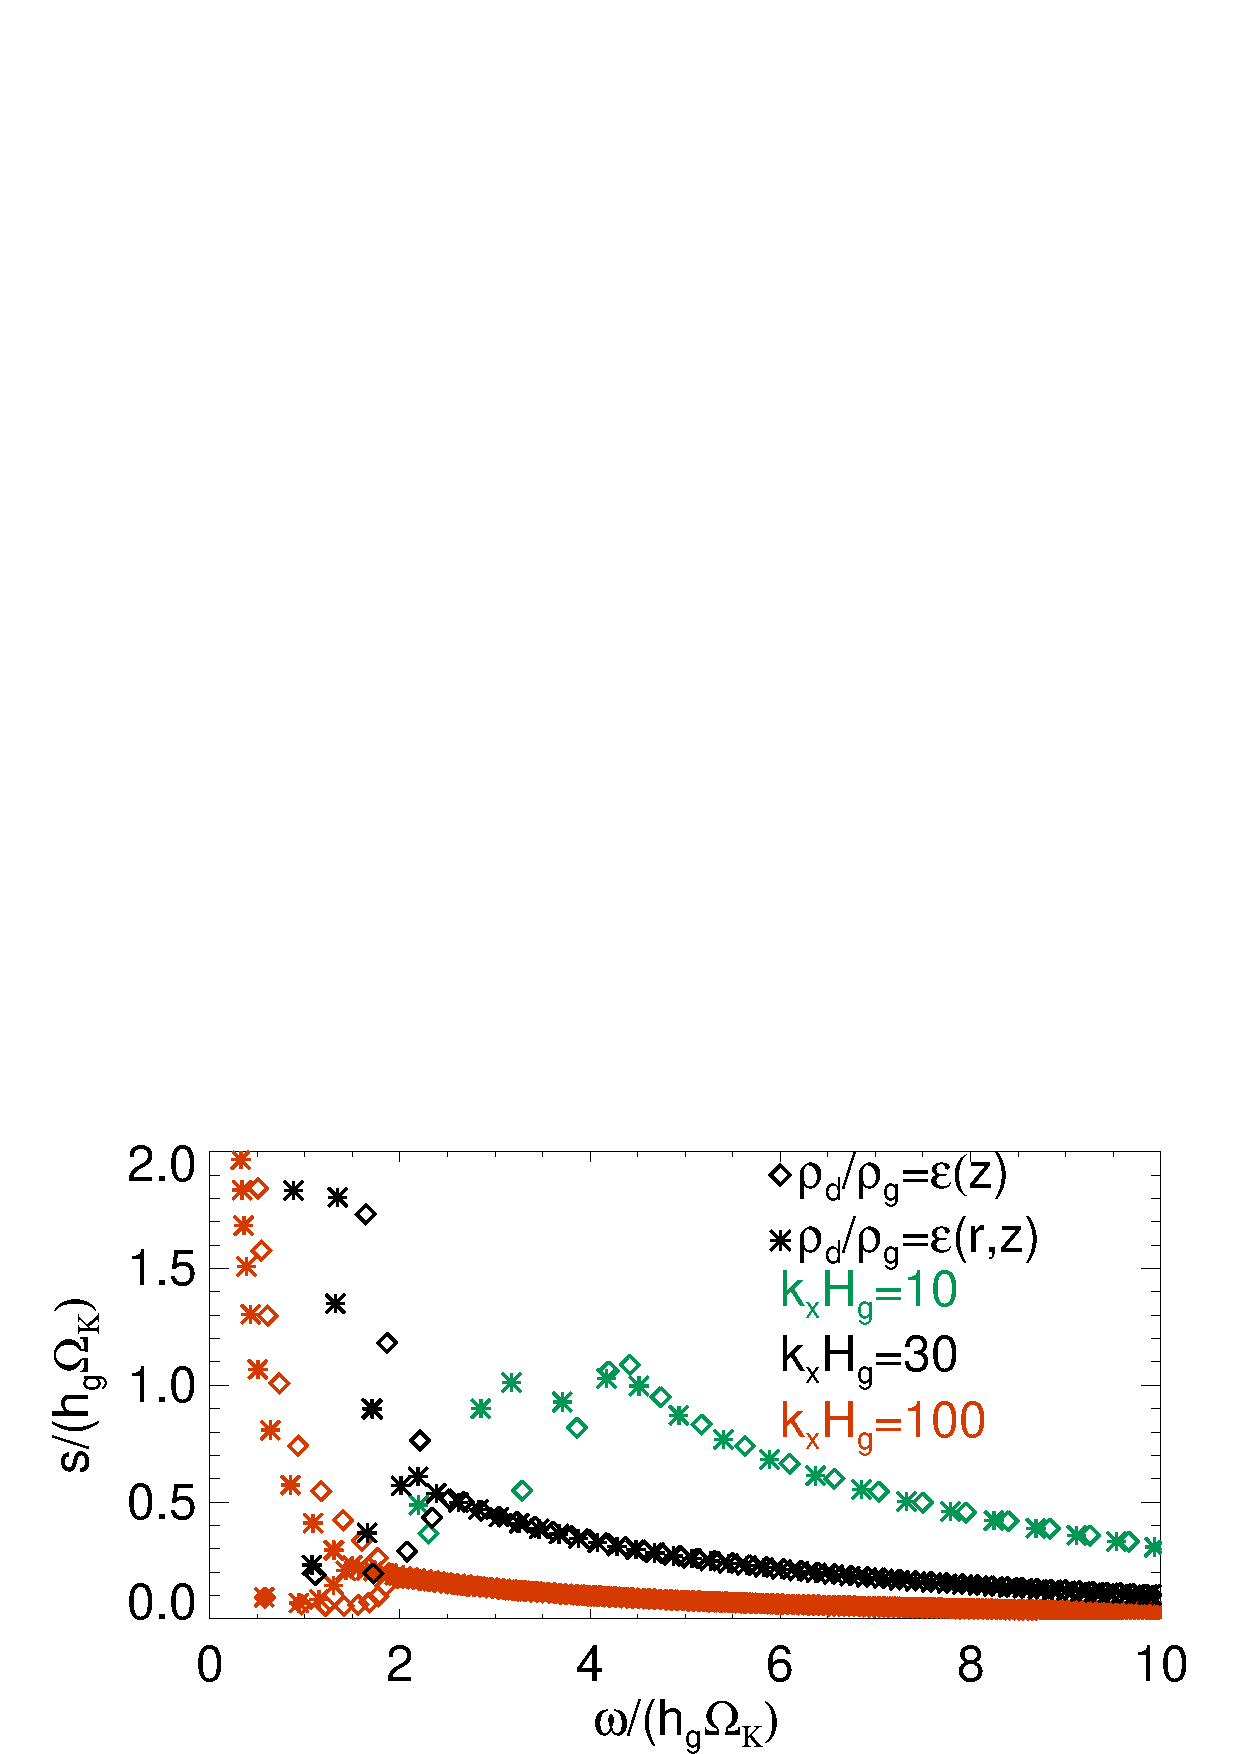
\includegraphics[width=\linewidth]{figures/compare_eigenvals_varHd} 
  \caption{Unstable VSI modes in the disk models of
    Fig. \protect\ref{compare_vshear_varHd}. { Diamonds (asterisks) 
    are mode frequencies for a disk with radially uniform (varying)
    dust-to-gas ratio. The radial wavenumbers are $k_xH_g = 10$
    (green),$k_xH_g = 30$ (black) and $k_xH_g = 100$ (orange). }
    \label{vsi_dust_varHd}
    }
\end{figure}

\subsection{Pure instability with vertically well-mixed
  dust}\label{vert_mixed} 

In \S\ref{iso_perfect} we found that for strictly isothermal
disks, a vertically-uniform dust-to-gas ratio can be unstable
if $d\epsilon/dr\neq0$.   
{
To demonstrate this numerically we set $q=0$ and $H_\mathrm{d}$ such
that $H_\epsilon=10^3\Hg$. We let $\rhod/\rhog \propto r^{-d}$
with different power indices $d$. The metalicity is fixed to $Z=0.03$.  
In these cases vertical shear $\p_z\Omega$ is 
attributed to the radially-varying dust-to-gas ratio (see
Eq. \ref{vshear2}).    
}

{ We show unstable modes in 
Fig. \ref{vert_mixed_modes}.} 
%In order to obtain appreciable growth   
%rates, we consider super-Solar metalicity $Z=0.03$ and high
%radial wavenumber $k_x\Hg=1800$. 
As expected from the discussion in
\S\ref{iso_perfect}, the disk admits purely growing modes with
$\omega=0$. This is distinct from the growing oscillations associated
with classic VSI discussed above. 

{ We find in smooth disks large 
  $k_x$ is needed for appreciable growth rates, e.g. $k_xH_g=1800$
  with $\rhod/\rhog\propto r^{-1}$. 
  Local shearing box simulations may 
  be required to study the non-linear evolution of such short 
  wavelengths \citep[e.g.][]{bai10b,yang16}. Alternatively, as shown in Fig. \ref{vert_mixed_modes},
  a rapidly varying dust-to-gas ratio permits dynamical instability at
  longer radial wavelengths, which might be resolvable in global disk 
  simulations. 
}

\begin{figure}
  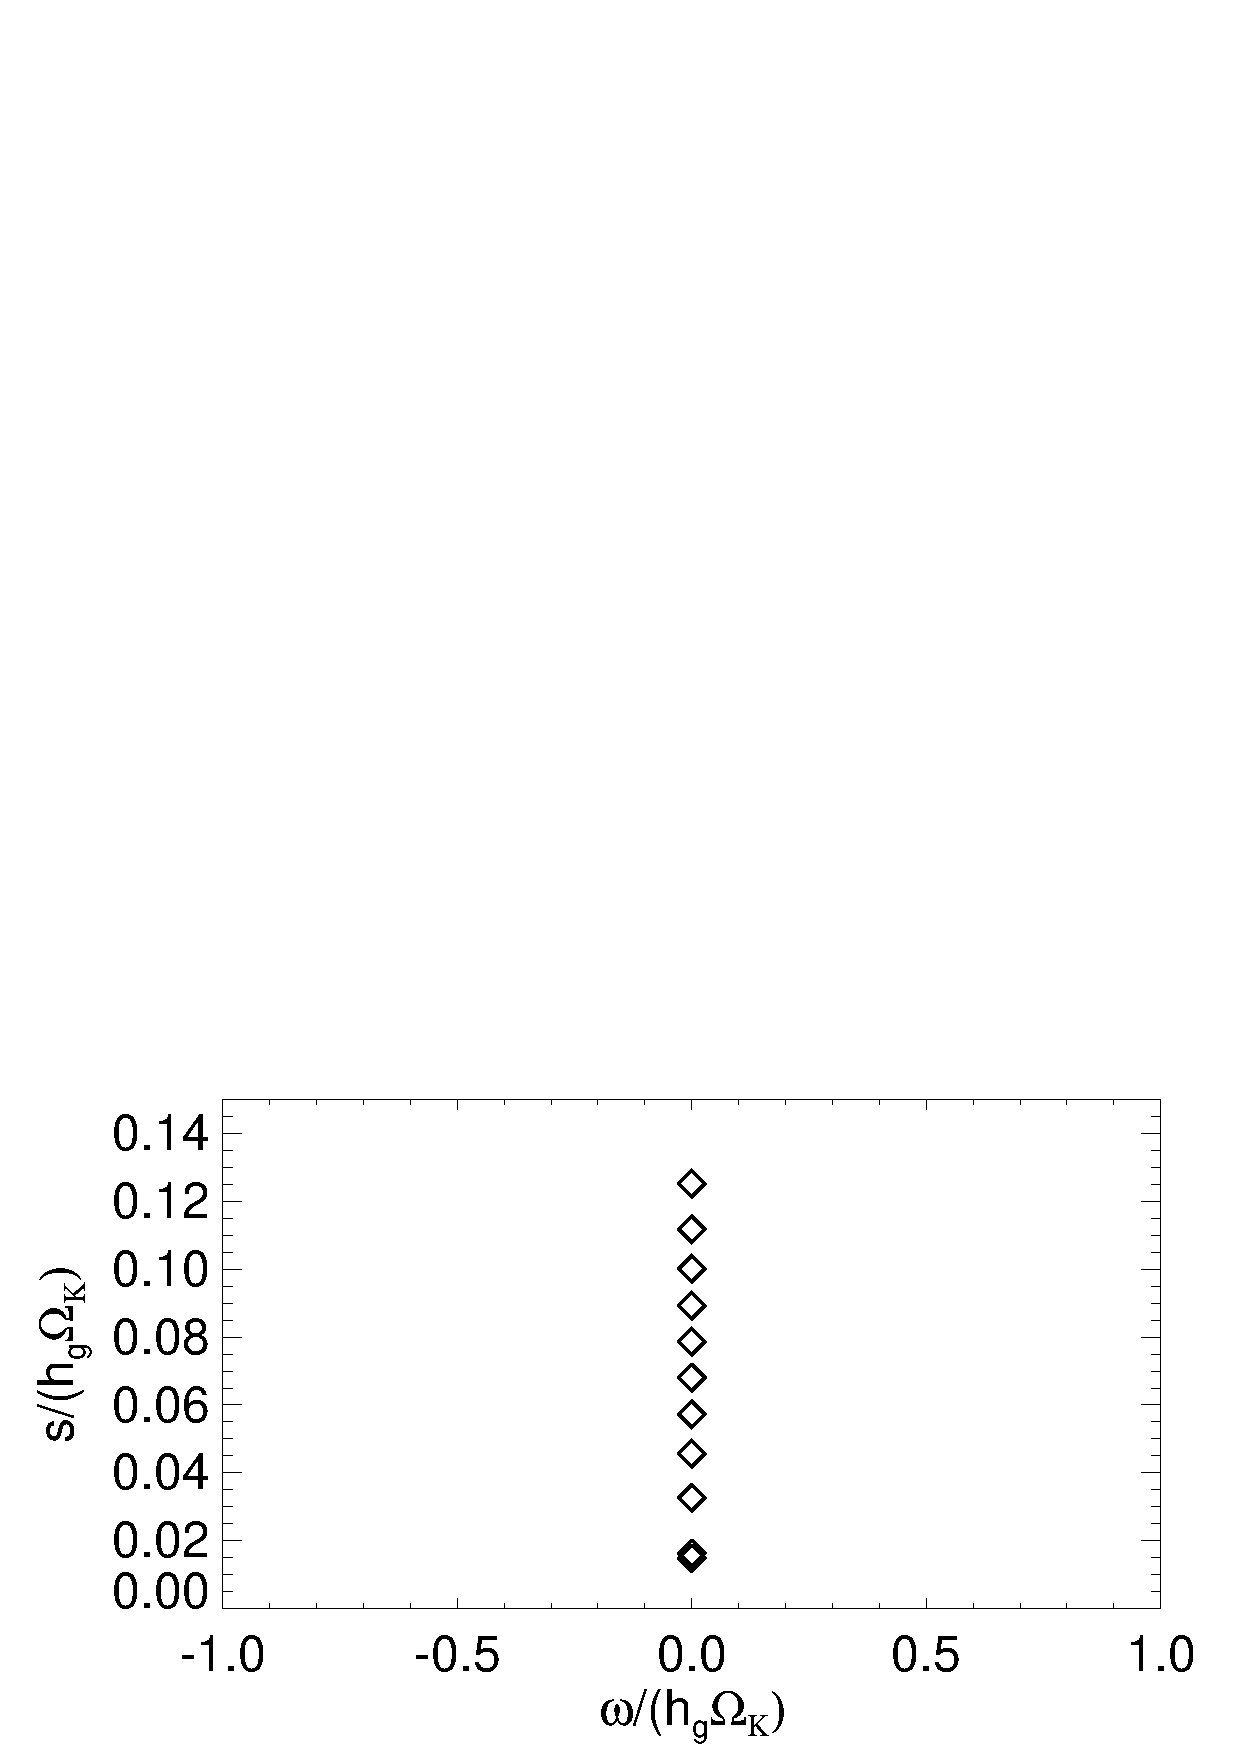
\includegraphics[width=\linewidth]{figures/vert_mixed_modes} 
  \caption{Purely growing modes in a strictly isothermal disk ($q=0$) with
    vertically uniform dust-to-gas ratio. The instability is due to 
    vertical shear $\p_z\Omega\neq0$ arising from radial variations in
    the dust-to-gas ratio, $d\epsilon/dr\neq 0$. \label{vert_mixed_modes}
    }
\end{figure}

%{\bf
%  \subsection{Implications for protoplanetary disks}
%dust settling, dust-induced buoyancy 
%The above calculations 
%radial d/g -> radial temp profile 
%}


